\documentclass[14pt, a4paper]{article}
\usepackage[russian]{babel}
\usepackage{graphicx}
\usepackage{layout}
\usepackage[14pt]{extsizes}
\usepackage{amssymb}
\usepackage{relsize}

\setcounter{tocdepth}{4}
\setcounter{secnumdepth}{4}

\usepackage{xcolor}
\usepackage{hyperref}

\usepackage{listings}

 % Цвета для гиперссылок
\definecolor{linkcolor}{HTML}{000000} % цвет ссылок
\definecolor{urlcolor}{HTML}{000000} %цвет гиперссылок

\hypersetup{pdfstartview=FitH,  linkcolor=linkcolor,urlcolor=urlcolor, colorlinks=true}

\definecolor{codegreen}{rgb}{0,0.6,0}
\definecolor{codegray}{rgb}{0.5,0.5,0.5}
\definecolor{codepurple}{rgb}{0.58,0,0.82}
\definecolor{backcolour}{rgb}{0.97,0.97,0.97}



%таблица
\lstdefinestyle{mystyle}{
    backgroundcolor=\color{backcolour},   
    commentstyle=\color{codegreen},
    keywordstyle=\color{magenta},
    numberstyle=\tiny\color{codegray},
    stringstyle=\color{codepurple},
    basicstyle=\ttfamily\footnotesize,
    breakatwhitespace=false,         
    breaklines=true,                 
    captionpos=b,                    
    keepspaces=true,
    frame=single,                                                    
    showspaces=false,                
    showstringspaces=false,
    showtabs=false,                  
    tabsize=2,
    mathescape=true
}

\lstset{style=mystyle, extendedchars=\true, literate=
{а}{ {\selectfont\char224} }1
{б}{ {\selectfont\char225} }1
{в}{ {\selectfont\char226} }1
{г}{ {\selectfont\char227} }1
{д}{ {\selectfont\char228} }1
{е}{ {\selectfont\char229} }1
{ё}{ {\"e} }1
{ж}{ {\selectfont\char230} }1
{з}{ {\selectfont\char231} }1
{и}{ {\selectfont\char232} }1
{й}{ {\selectfont\char233} }1
{к}{ {\selectfont\char234} }1
{л}{ {\selectfont\char235} }1
{м}{ {\selectfont\char236} }1
{н}{ {\selectfont\char237} }1
{о}{ {\selectfont\char238} }1
{п}{ {\selectfont\char239} }1
{р}{ {\selectfont\char240} }1
{с}{ {\selectfont\char241} }1
{т}{ {\selectfont\char242} }1
{у}{ {\selectfont\char243} }1
{ф}{ {\selectfont\char244} }1
{х}{ {\selectfont\char245} }1
{ц}{ {\selectfont\char246} }1
{ч}{ {\selectfont\char247} }1
{ш}{ {\selectfont\char248} }1
{щ}{ {\selectfont\char249} }1
{ъ}{ {\selectfont\char250} }1
{ы}{ {\selectfont\char251} }1
{ь}{ {\selectfont\char252} }1
{э}{ {\selectfont\char253} }1
{ю}{ {\selectfont\char254} }1
{я}{ {\selectfont\char255} }1
{А}{ {\selectfont\char192} }1
{Б}{ {\selectfont\char193} }1
{В}{ {\selectfont\char194} }1
{Г}{ {\selectfont\char195} }1
{Д}{ {\selectfont\char196} }1
{Е}{ {\selectfont\char197} }1
{Ё}{ {\"E} }1
{Ж}{ {\selectfont\char198} }1
{З}{ {\selectfont\char199} }1
{И}{ {\selectfont\char200} }1
{Й}{ {\selectfont\char201} }1
{К}{ {\selectfont\char202} }1
{Л}{ {\selectfont\char203} }1
{М}{ {\selectfont\char204} }1
{Н}{ {\selectfont\char205} }1
{О}{ {\selectfont\char206} }1
{П}{ {\selectfont\char207} }1
{Р}{ {\selectfont\char208} }1
{С}{ {\selectfont\char209} }1
{Т}{ {\selectfont\char210} }1
{У}{ {\selectfont\char211} }1
{Ф}{ {\selectfont\char212} }1
{Х}{ {\selectfont\char213} }1
{Ц}{ {\selectfont\char214} }1
{Ч}{ {\selectfont\char215} }1
{Ш}{ {\selectfont\char216} }1
{Щ}{ {\selectfont\char217} }1
{Ъ}{ {\selectfont\char218} }1
{Ы}{ {\selectfont\char219} }1
{Ь}{ {\selectfont\char220} }1
{Э}{ {\selectfont\char221} }1
{Ю}{ {\selectfont\char222} }1
{Я}{ {\selectfont\char223} }1
}

% \lstset{style=mystyle}

%Разметка страницы
\oddsidemargin = 0pt
\marginparwidth = 45pt 
\textwidth = 467pt
\textheight = 716pt
\topmargin = 0pt 
\footskip = 30pt 
\headheight = 0pt 
\headsep = 0pt 

\begin{document}
\begin{titlepage}
    \topmargin=216pt
    \newpage
    \hangindent=0.7cm
    \huge ИУ-10\\
    Системное\\
    Программное\\
    Обеспечение\\
    Администрирование Linux\\
    \textbf{Работа с Web и TFTP сервером}

    \vspace{10cm}

    \begin{center}
        \small\textit{Москва, 2022}
    \end{center}
\end{titlepage}

\section*{На этом уроке} 
\addcontentsline{toc}{section}{На этом уроке}

\begin{enumerate}
    \item Обзор репозиториев, файлов конфигурации
    \item Установка и базовая настройка NGINX
    \item Установка и базовая настройка TFTP-server
\end{enumerate}

\tableofcontents
\newpage


\section*{Управление ПО в Linux} 
\addcontentsline{toc}{section}{Управление ПО в Linux}

В Ubuntu программное обеспечение делится на четыре вида по типу лицензирования и уровню
поддержки:
\begin{enumerate}
    \item \textbf{Main} — свободное ПО, официально поддерживаемое компанией Cano- nical.
    \item \textbf{Restricted} — проприетарное ПО (в основном драйверы устройств), официально
    поддерживаемое компанией Canonical.
    \item \textbf{Universe} — свободное ПО, официально не поддерживаемое компанией Canonical, но
    поддерживаемое сообществом пользователей.
    \item \textbf{Multiverse} — проприетарное ПО, не поддерживаемое компанией Cano- nical.
\end{enumerate}

Все перечисленные виды программного обеспечения представляют из себя набор файлов и
библиотек, объединенных для выполнения определенного функционала, которые мы можем
установить. Это объединение называется пакетом.

\subsection*{Репозитории и управление репозиториями} 
\addcontentsline{toc}{subsection}{Репозитории и управление репозиториями}

Пакеты располагаются в своих хранилищах - репозиториях. Репозиторий может быть размещён
локально, может находиться на носителе (флешке, DVD-диске), но чаще всего он размещён в
интернете. Условно репозитории можно разделить на три группы:

\begin{enumerate}
    \item \textbf{Стандартные репозитории} — это репозитории, поддерживаемые разработчиками
    операционных систем. Включают в себя стабильные версии программного обеспечения.
    Зачастую эти версии отстают на несколько шагов от последних версий пакетов.
    \item \textbf{Дополнительные репозитории} — репозитории, поддерживаемые разработчиками
    программного обеспечения. Включают в себя последние стабильные версии ПО. Зачастую
    узкоспециализированы под конкретный пакет и библиотеки, необходимые для этого пакета.
    \item \textbf{Неофициальные репозитории} — репозитории, созданные сообществом или одним
    человеком. Могут содержать в себе как последние стабильные, так и тестируемые версии
    программного обеспечения.
\end{enumerate}

\noindent Официальные репозитории Ubuntu делятся на следующие типы:
\begin{enumerate}
    \item \textbf{\$release} — пакеты на момент выхода релиза.
    \item \textbf{\$release-security} — пакеты критических обновлений безопасности.
    \item \textbf{\$release-updates} — пакеты обновления системы, то есть более поздние версии ПО,
    вышедшие уже после релиза.
    \item \textbf{\$release-backports} — пакеты более новых версий ПО, которое доступно только в
    нестабильных версиях Ubuntu.
    \item \textbf{partner} — репозиторий, содержащий ПО компаний-партнёров Cano- nical.
\end{enumerate}

Информация о подключённых репозиториях в Ubuntu хранится в каталоге \textbf{/etc/apt/}, в файле
\textbf{sources.list}. \textbf{Важно!} \underbar{\textit{Репозитории защищают}} \\ 
\underbar{\textit{от подмены при помощи сверки цифровых подписей репозитория и кли-}} \\
\underbar{\textit{ента. В репозитории хранится закрытая часть ключа, у клиента \ \ — }} \\
\underbar{\textit{открытая часть ключа.}}\\

В Ubuntu репозитории можно подключить тремя способами: используя графический интерфейс, путём
редактирования файла \textbf{/etc/apt/source.} \textbf{list} или добавления файла в каталог \textbf{/etc/apt/source.list.d/} и
используя утилиту apt. Рассмотрим два последних варианта.

\subsubsection*{Добавление репозитория через добавления файла} 
\addcontentsline{toc}{subsubsection}{Добавление репозитория через добавления файла}

В текстовом редакторе открываем файл \textbf{/etc/apt/source.list.d/repo.list} и в конце файла вводим строку
вида:

\vspace{0.3cm}
\begin{lstlisting}
deb http://адрес_репозитория версия_дистрибутива ветки
\end{lstlisting}
\vspace{0.2cm}

Например, добавим репозиторий nginx, для этого создадим в каталоге /etc/apt/source.list.d/ файл
nginx.list следующего содержания:

\vspace{0.3cm}
\begin{lstlisting}
deb http://nginx.org/packages/ubuntu focal nginx
\end{lstlisting}
\vspace{0.2cm}

Здесь nginx — название ветки, содержащей пакеты, необходимые для установки nginx, а focal — это
кодовое имя версии. Узнать его можно с помощью команды \colorbox{backcolour}{lsb\_release -a}.

\vspace{0.3cm}
\begin{lstlisting}
root@server:$\sim$# lsb_release -a
No LSB modules are available.
Distributor ID:    Ubuntu
Description: Ubuntu 20.04.1 LTS
Release:     20.04
Codename:    focal
\end{lstlisting}
\vspace{0.2cm}

Следующий шаг — это установка публичного ключа репозитория, для этого нужна команда \textbf{apt-key}.
Скачиваем при помощи \textbf{curl} наш ключ и передаём через pipe утилите \textbf{apt-key}:

\vspace{0.3cm}
\begin{lstlisting}
curl -fsSL https://nginx.org/keys/nginx_signing.key | sudo apt-key add -
\end{lstlisting}
\vspace{0.2cm}

И последний шаг — это обновление информации о пакетах \textbf{sudo apt update} и установка пакета 
\textbf{sudo apt install nginx -y}.\\

Создание файлов c репозиториями и размещение их в каталоге \textbf{/etc/} \textbf{source.list.d/} удобно тем, что мы
можем обновить информацию о пакетах из конкретного репозитория \textbf{apt update repo\_name}.

\subsubsection*{Добавление репозитория, используя команду apt-add-repository} 
\addcontentsline{toc}{subsubsection}{Добавление репозитория, используя команду apt-add-repository}

Эта команда автоматически создаёт записи в файле \textbf{/etc/apt/sources.list} или создаёт файл
репозитория в каталоге \textbf{/etc/apt/sources.list.d/}, а также может удалять информацию о репозиториях.
Чаще всего эта утилита используется для добавления PPA-репозиториев.\\

PPA-репозитории находятся \href{https://launchpad.net/}{на сайте Launchpad.net}, который поддерживается компанией Canonical.
Утилита автоматически находит строку для записи в файл репозитория, скачивает и импортирует
ключи. Рассмотрим добавление репозитория nginx с использованием PPA-репозитория:

\vspace{0.3cm}
\begin{lstlisting}
apt-add-repository ppa:nginx/stable
\end{lstlisting}
\vspace{0.2cm}

Здесь утилите apt-add-repository мы говорим, что подключаем PPA-репозиторий, поддерживаемый
группой nginx, и подключаем стабильную версию. Утилита автоматически создаст файл
\textbf{/etc/apt/sources.list.d/} \textbf{nginx-ubuntu-stable-bionic.list} с содержимым, которое мы можем просмотреть
при помощи команды cat:

\vspace{0.3cm}
\begin{lstlisting}
cat /etc/apt/sources.list.d/nginx-ubuntu-stable-focal.list

"deb http://ppa.launchpad.net/nginx/stable/ubuntu focal main"
\end{lstlisting}
\vspace{0.2cm}

Утилита импортирует ключи и обновит список пакетов.

\subsection*{Управление пакетами} 
\addcontentsline{toc}{subsection}{Управление пакетами}

В Ubuntu управление пакетами осуществляется тремя способами: с использованием утилиты apt, dpkg
или snap. Разберем первые две как наиболее популярные.

\newpage

\subsubsection*{Управление пакетами через утилиту apt} 
\addcontentsline{toc}{subsubsection}{Управление пакетами через утилиту apt}

\textbf{apt} - пакетный менеджер, который включает в себя набор утилит для управления пакетами. Он
позволяет осуществлять поиск, установку и удаление пакетов, обновлять операционную систему,
подключать репозитории. Подключение репозиториев с использованием \textbf{apt} было рассмотрено в
предыдущей части. Рассмотрим параметры утилиты \textbf{apt} для управления пакетами:

\begin{itemize}
    \item \colorbox{backcolour}{apt search package\_name} — поиск пакета;
    \item \colorbox{backcolour}{apt show package\_name} — посмотреть информацию о пакете;
    \item \colorbox{backcolour}{apt install package\_name -y} — установить пакет;
    \item \colorbox{backcolour}{apt install package\_name1 package\_name2 -y} — установить два пакета;
    \item \colorbox{backcolour}{apt remove package\_name} — удалить пакет, при этом сохранятся файлы с настройками;
    \item \colorbox{backcolour}{apt purge package\_name} — полностью удалить пакет, включая конфигурационные файлы;
    \item \colorbox{backcolour}{apt upgrade} — обновить все установленные пакеты;
    \item \colorbox{backcolour}{apt update} — обновить информацию о пакетах в репозиториях, указанных в настройках.
\end{itemize}

\subsubsection*{Управление пакетами через утилиту dpkg} 
\addcontentsline{toc}{subsubsection}{Управление пакетами через утилиту dpkg}

\textbf{Dpkg} — пакетный менеджер в Debian-подобных системах. Главное отличие от утилиты \textbf{apt} состоит в
том, что \textbf{dpkg} работает только с локальными пакетами, он не умеет искать и устанавливать пакеты с
репозиториев. Основные параметры утилиты \textbf{dpkg}:

\begin{itemize}
    \item \colorbox{backcolour}{dpkg -l} — просмотр списка пакетов;
    \item \colorbox{backcolour}{dpkg -i package\_name} — установить пакет или группу пакетов;
    \item \colorbox{backcolour}{dpkg -r package\_name} — удалить пакет или группу пакетов.
\end{itemize}

\newpage

\section*{TFTP сервер} 
\addcontentsline{toc}{section}{TFTP сервер}

TFTP или Trivial File Transfer Protocol - это протокол, который можно использовать для быстрого
перемещения \underbar{\textit{небольших файлов}}. В отличии от FTP, TFTP работает поверх UDP (порт 69) и в
большинстве случаев не использует имя пользователя и пароль. При этом файл передается частями
по 512 байт с подтверждением каждого, что замедляет передачу больших файлов.\\

TFTP используется там, где безопасность не требуется. Вместо этого вам нужен способ легко
выгружать файлы на сервер и скачивать их с сервера. Коммутаторы и маршрутизаторы используют
протокол TFTP для хранения файлов конфигурации и образов ПО в целях резервного копирования.
Протоколы сетевой загрузки, такие как BOOTP, PXE используют этот протокол для загрузки
операционных систем по сети. Многие электронные платы и микропроцессоры также используют
TFTP для загрузки прошивки в чип.\\

Давайте рассмотрим установку и использование пакеты \textbf{tftpd-hpa} в качестве TFTP-сервера.\\

Установим,включим и добавим службу в автоматическую загрузку.

\vspace{0.3cm}
\begin{lstlisting}
root@server:$\sim$# apt-get install tftpd-hpa
Reading package lists... Done
Building dependency tree
Reading state information... Done
...
root@server:$\sim$# systemctl start tftpd-hpa.service
root@server:$\sim$# systemctl enable tftpd-hpa.service
tftpd-hpa.service is not a native service, redirecting to systemd-sysv-
install.
Executing: /lib/systemd/systemd-sysv-install enable tftpd-hpa
root@server:$\sim$#
root@server:$\sim$#
root@server:$\sim$# systemctl status tftpd-hpa.service
$\bullet$ tftpd-hpa.service - LSB: HPA's tftp server
    Loaded: loaded (/etc/init.d/tftpd-hpa; generated)
    Active: active (running) since Wed 2021-01-13 11:50:06 UTC; 2min 31s ago
      Docs: man:systemd-sysv-generator(8)
     Tasks: 1 (limit: 2282)
    Memory: 616.0K
    CGroup: /system.slice/tftpd-hpa.service
               $ {^\mathlarger{\mathlarger{{\mathlarger{\llcorner}}}}} $4642 /usr/sbin/in.tftpd --listen --user tftp --address :69
--secure /srv/tftp
$$
\end{lstlisting}
\newpage

\begin{lstlisting}
Jan 13 11:50:06 server systemd[1]: Starting LSB: HPA's tftp server...
Jan 13 11:50:06 server tftpd-hpa[4634]: * Starting HPA's tftpd in.tftpd
Jan 13 11:50:06 server tftpd-hpa[4634]:   ...done.
Jan 13 11:50:06 server systemd[1]: Started LSB: HPA's tftp server.
root@server:$\sim$#
$$
\end{lstlisting}
\vspace{0.2cm}

Конфигурация сервера находится в /etc/default/tftpd-hpa и содержит следующие параметры.

\begin{itemize}
    \item[-] \textbf{TFTP\_USERNAME="tftp"}. Пользователь, от имени которого будет запущен сервис, 
    \underbar{\textbf{а не логин доступа к серверу}}.
    \item[-] \textbf{TFTP\_DIRECTORY="/srv/tftp"}. Каталог, доступный по tftp.
    \item[-] \textbf{TFTP\_ADDRESS=":69"}. Порт, на котором работает протокол.
    \item[-] \textbf{TFTP\_OPTIONS="$--$secure"}. Эта переменная устанавливает изменение каталога \ TFTP \ на тот,
    который установлен \ в \ переменной \\ \textbf{TFTP\_DIRECTORY} при подключении к серверу TFTP. Это
    функция безопасности. Если этот параметр не установлен, после подключения придется
    установить каталог вручную. Это очень хлопотно и небезопасно. 
\end{itemize}

Добавим опцию \textbf{$--$create}, так как без нее на сервер невозможно будет загружать новые файлы.

\vspace{0.3cm}
\begin{lstlisting}
root@server:$\sim$# cat /etc/default/tftpd-hpa
# /etc/default/tftpd-hpa

TFTP_USERNAME="tftp"
TFTP_DIRECTORY="/srv/tftp"
TFTP_ADDRESS=":69"
TFTP_OPTIONS="--secure --create"
\end{lstlisting}
\vspace{0.2cm}

Для корректного доступа к файлам сменим владельца и группу папки \textbf{/srv/tftp}. Рестартуем сервис и
создадим файл в папке.

\vspace{0.3cm}
\begin{lstlisting}
root@server:$\sim$# chown tftp:tftp /srv/tftp/
root@server:$\sim$# systemctl restart tftpd-hpa.service
root@server:$\sim$# systemctl status tftpd-hpa.service
$\bullet$ tftpd-hpa.service - LSB: HPA's tftp server
    Loaded: loaded (/etc/init.d/tftpd-hpa; generated)
    Active: active (running) since Wed 2021-01-13 12:22:53 UTC; 4s ago
      Docs: man:systemd-sysv-generator(8)
         Process: 4981 ExecStart=/etc/init.d/tftpd-hpa start (code=exited,
status=0/SUCCESS)
     Tasks: 1 (limit: 2282)
    Memory: 492.0K
    CGroup: /system.slice/tftpd-hpa.service
               $ {^\mathlarger{\mathlarger{{\mathlarger{\llcorner}}}}} $4998 /usr/sbin/in.tftpd --listen --user tftp --address :69
--secure --create /srv/tftp
\end{lstlisting}
\newpage

\begin{lstlisting}
    
Jan 13 12:22:53 server systemd[1]: Starting LSB: HPA's tftp server...
Jan 13 12:22:53 server tftpd-hpa[4981]: * Starting HPA's tftpd in.tftpd
Jan 13 12:22:53 server tftpd-hpa[4981]: ...done.
Jan 13 12:22:53 server systemd[1]: Started LSB: HPA's tftp server.
root@server:$\sim$# echo "Some data on TFTP!"> /srv/tftp/tftp_data
$$
\end{lstlisting}
\vspace{0.2cm}

Для доступа к TFTP-серверу понадобится клиентская программа TFTP. Она вам понадобится только
для тестирования, потому что на устройствах, которые будут использовать TFTP-сервер, скорее всего
уже будет установлена клиентская программа. Например, почти на всех маршрутизаторах и
коммутаторах уже есть клиент.

\vspace{0.3cm}
\begin{lstlisting}
user-client_machine:$\sim$ user$\textdollar$ tftp 192.168.1.84
tftp> status
Connected to 192.168.1.84.
Mode: netascii Verbose: off Tracing: off
Rexmt-interval: 5 seconds, Max-timeout: 25 seconds
tftp> get tftp_data
getting from 192.168.1.84:tftp_data to tftp_data [netascii]
Received 20 bytes in 0.0 seconds [inf bits/sec]
Sent 12 bytes in 0.0 seconds
tftp> put local_data
tftp> quit
user-client_machine:$\sim$ user$\textdollar$ cat tftp_data
Some data on TFTP!
$$
\end{lstlisting}
\vspace{0.2cm}

Таким образом мы можем загружать и скачивать файлы, настройка сервера закончена.

\vspace{0.3cm}
\begin{lstlisting}
root@server:~# ls -la /srv/tftp/
total 16
drwxr-xr-x 2 tftp tftp 4096 Jan 13 12:32 .
drwxr-xr-x 3 root root    4096 Jan 13 11:49 ..
-rw-rw-rw- 1 tftp tftp      11 Jan 13 12:32 local_data
-rw-r--r-- 1 root root      19 Jan 13 12:26 tftp_data
\end{lstlisting}

\section*{Web сервер} 
\addcontentsline{toc}{section}{Web сервер}

Веб-сервер — сервис, принимающий HTTP-запросы и выдающий ответы, как правило, содержащие
HTML-код (но могут присутствовать и двоичные файлы).\\

HTTP сам по себе - это простой текстовый протокол, позволяющий запросить у веб-сервера
информацию, а серверу ее отдать. HTTP-протокол позволяет передавать заголовки, на основе
которых выполняется обработке данных. HTTP-клиент, в роли которого, как правило, выступает
браузер, сообщает информацию о себе через user аgent. curl и wget тоже имеют user agent, таким
образом, не каждый HTTP-клиент — браузер. Веб-сервер сообщает информацию о себе,
метаинформацию о документе, кодировку и тип содержимого (MIME-type), что позволит клиенту
корректно раскодировать информацию.\\

Существует несколько типов запросов, но наиболее часто применяются GET и POST.\\

GET служит для запроса страницы. Как правило, в качестве адреса ресурса в GET передаётся путь к
файлу относительно веб-директории. Например, \textbf{/articles/article.html}.\\

С помощью POST отправляются новые файлы на веб-сервер (upload), записи на форумах и блогах,
логин и пароль для входа в ту или иную систему.\\

Протокол HTTP, как правило, работает через TCP-сессию. Поэтому для приёма нескольких
одновременных соединений веб-сервер должен использовать процессы или потоки.

\subsection*{Nginx} 
\addcontentsline{toc}{subsection}{Nginx}

Одним из самых распространенных Веб-серверов является NGINX, позиционируется как простой,
быстрый и надежный сервер. В целом, NGINX скорее веб-прокси, чем полноценный веб-сервер, так
как для работы с динамическим контентом используются внешние приложения.\\

Nginx использует следующий механизм: он создает один мастер-процесс и один или более
процессов-воркеров (worker). Как правило, на одном CPU используется один воркер, но может
применяться и больше, например при интенсивном вводе-выводе. Все входящие подключения
распределяются по воркерам. Каждый воркер использует одну очередь и низкоуровневые механизмы,
что позволяет обработать довольно значительное число соединений. Используя низкоуровневые
возможности операционной системы, и вместо того, чтобы доверять переключение между задачами
процессорного времени с помощью потоков, Nginx самостоятельно реализует обработку
одновременных соединений. Этим достигается высокое быстродействие, отказоустойчивость, но
именно поэтому Nginx может работать только со статическим содержимым. Чтобы использовать
динамическое содержимое, генерируемое скриптами, Nginx может получать результаты выполнения
от сторонних приложенией, например PHP, работающего через модуль php-fpm. Так как в таком
случае скрипты выполняются в другом процессе, работа Nginx безопасна. Nginx будет хорошо
работать, если файлы, к которым обращаются HTTP-запросы, не блокируются другими
приложениями.\\

Для работы nginx нам понадобится свободный 80 порт, поэтому убедитесь что он не занят другим
процессом.

\vspace{0.3cm}
\begin{lstlisting}
root@server:$\sim$# netstat -tulapn | grep 80
root@server:$\sim$#
\end{lstlisting}
\vspace{0.2cm}

В первой части урока мы добавили репозиторий, содержащий нужный нам пакет, поэтому осталось
только его установить и запустить.

\vspace{0.3cm}
\begin{lstlisting}
root@server:$\sim$# apt-get update
root@server:$\sim$# apt-get install nginx
root@server:$\sim$# systemctl start nginx.service
root@server:$\sim$# systemctl status nginx.service
$\bullet$ nginx.service - A high performance web server and a reverse proxy server
     Loaded: loaded (/lib/systemd/system/nginx.service; enabled; vendor 
preset: enabled)
     Active: active (running) since
$$
\end{lstlisting}
\vspace{0.2cm}

Nginx доступен с набором настроек по умолчанию и стартовая страница выглядит следующим
образом.

\begin{figure}[h]
    \centering
    \scalebox{1}{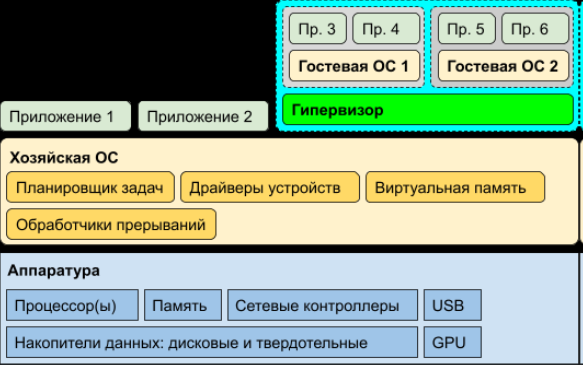
\includegraphics[width=1\textwidth]{1.png}}\\ 
    \small\textit{Рис.1 - Стартовая страница NGINX}  
    \label{framework} 
\end{figure}

\subsubsection*{Базовые настройки} 
\addcontentsline{toc}{subsubsection}{Базовые настройки}

Файлы конфигурации находятся в каталоге \textbf{/etc/nginx}. Основным является является
\textbf{/etc/nginx/nginx.conf}.

\newpage

\begin{lstlisting}
root@server:~# cat /etc/nginx/nginx.conf | grep -vP '^\s*#|^$\textdollar$'
user www-data;
worker_processes auto;
pid /run/nginx.pid;
include /etc/nginx/modules-enabled/*.conf;
events {
      worker_connections 768;
}
http {
      sendfile on;
      tcp_nopush on;
      types_hash_max_size 2048;
      include /etc/nginx/mime.types;
      default_type application/octet-stream;
      ssl_protocols TLSv1 TLSv1.1 TLSv1.2 TLSv1.3; # Dropping SSLv3, ref: 
POODLE
      ssl_prefer_server_ciphers on;
      access_log /var/log/nginx/access.log;
      error_log /var/log/nginx/error.log;
      gzip on;
      include /etc/nginx/conf.d/*.conf;
      include /etc/nginx/sites-enabled/*;
}
\end{lstlisting}
\vspace{0.2cm}

Основными понятиями в конфигурации являются контекст и директива. Контекст - это набор директив,
заключенных в фигурные скобки.

\vspace{0.3cm}
\begin{lstlisting}
events {
      worker_connections 768;
}
\end{lstlisting}
\vspace{0.2cm}

В данном примере \colorbox{backcolour}{worker\_connections} находятся в контексте \colorbox{backcolour}{events}. 
При этом \colorbox{backcolour}{events} является
директивой основного контекста. \textbf{Примечание!} 
\underbar{\textit{Одинаковые директивы могут находиться в разных контекстах.В}} \\
\underbar{\textit{этом случае будет применяться последняя.Далее будут приведены при-}} \\
\underbar{\textit{меры таковых}}\\

Начнем составлять конфигурацию с нуля.

\vspace{0.3cm}
\begin{lstlisting}
events {}

http{

server {
        listen 80;
        server_name 192.168.1.84;
    
        }
}
\end{lstlisting}
\vspace{0.2cm}

\begin{itemize}
    \item[-] \colorbox{backcolour}{events \{\}} относится к обработке соединений, она должна существовать всегда, но может
    быть пустой
    \item[-] \colorbox{backcolour}{http} описывает протокол HTTP.NGINX может обрабатывать и почтовые запросы (директива
    mail)
    \item[-] \colorbox{backcolour}{listen} указывает, на каком порту необходимо открыть соединение
    \item[-] \colorbox{backcolour}{server\_name} проверяет значение HTTP-заголовка “Host”. В данный момент стоит указать IP
    адрес нашего сервера Linux.
\end{itemize}

Проверим конфигурацию на ошибки и перечитаем ее.

\vspace{0.3cm}
\begin{lstlisting}
root@server:$\sim$# nginx -t
nginx: the configuration file /etc/nginx/nginx.conf syntax is ok
nginx: configuration file /etc/nginx/nginx.conf test is successful
root@server:$\sim$# systemctl reload nginx.service
$$
\end{lstlisting}
\vspace{0.2cm}

Добавим директивы \colorbox{backcolour}{location},определяющие шаблоны, по которым ищут совпадения запроса после
“/” (слэш). В перед описанием шаблона может ничего не стоять, тогда шаблон будет означать
префикс, = точное совпадение шаблона, $\sim$ регулярное выражение, * case insensitive .

\vspace{0.3cm}
\begin{lstlisting}
events {}

http{

server {
        listen 80;
        server_name 192.168.1.84;
         location /hello {
                        return 200 'Hello World!';
                }
         location ~*/hi[0-9] {
                        return 200 'Hi There!';
                }
        }
}
\end{lstlisting}
\vspace{0.2cm}

В браузере мы увидим совпадение первого


\begin{figure}[h]
    \centering
    \scalebox{0.9}{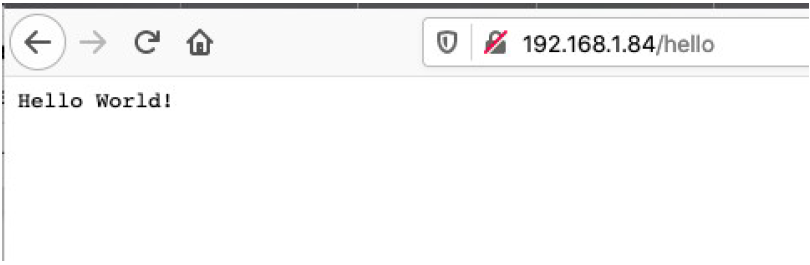
\includegraphics[width=1\textwidth]{2.png}}\\ 
    \label{framework} 
\end{figure}

\newpage

\begin{figure}[h]
    \centering
    \scalebox{0.9}{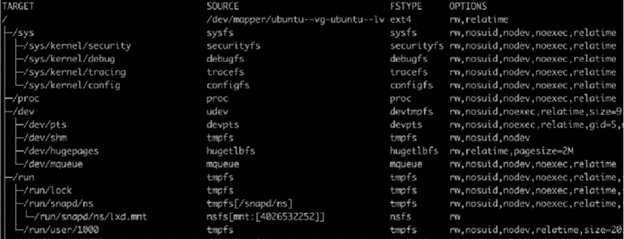
\includegraphics[width=1\textwidth]{3.png}}\\ 
    \small\textit{Рис2-3. Работа директивы location}   
    \label{framework} 
\end{figure}

\subsubsection*{Статические файлы} 
\addcontentsline{toc}{subsubsection}{Статические файлы}

Директива \colorbox{backcolour}{root} определяет корневой каталог, который будет использоваться для поиска файла.
Чтобы получить путь к запрошенному файлу, NGINX добавляет URI запроса к пути, указанному в
корневой директиве. Директива может быть размещена на любом уровне в контексте \colorbox{backcolour}{http}, \colorbox{backcolour}{server}
или \colorbox{backcolour}{location}.

\vspace{0.3cm}
\begin{lstlisting}
root@server:$\sim$# cat /etc/nginx/nginx.conf
events {}

http{ 
    
server {
        listen 80;
        server_name 192.168.1.84;
        root /srv/www;
        location /hello {
                        return 200 'Hello World!';
                }
        location ~*/hi[0-9] {
                        return 200 'Hi There!';
                }
        }
}
root@server:$\sim$# echo "Web data!" > /srv/www/web_data
root@server:$\sim$#
root@server:$\sim$# wget http://192.168.1.84:/web_data
--2021-01-13 14:30:19-- http://192.168.1.84/web_data
Connecting to 192.168.1.84:80... connected.
HTTP request sent, awaiting response... 200 OK
Length: 10 [text/plain]
Saving to: 'web_data'

web_data
100%[=====================================================================
==========>]      10 --.-KB/s     in 0s

2021-01-13 14:30:19 (1024 KB/s) - 'web_data' saved [10/10]

root@server:$\sim$# cat web_data
Web data!
\end{lstlisting}
\newpage

Мы можем создать отдельные папки под хранение файлов конфигураций и образов, программного
обеспечения. Для того, чтобы не запоминать весь путь, а опираться на расширения запрашиваемых
файлов, в разных контекстах \colorbox{backcolour}{location} использовать требуемую директиву \colorbox{backcolour}{root}.

\vspace{0.3cm}
\begin{lstlisting}
root@server:$\sim$# mkdir /srv/www/conf
root@server:$\sim$# mkdir /srv/www/iso
root@server:$\sim$#
root@server:$\sim$# cat /etc/nginx/nginx.conf
events {}

http{ 
    
server {
        listen 80;
        server_name 192.168.1.84;
        location $\sim$ \.cfg$\textdollar$ {
            root /srv/www/conf;
                }
        location $\sim$
            \.iso$\textdollar$ { root
            /srv/www/iso;
                }
        }
}
\end{lstlisting}
\vspace{0.2cm}

В данном примере iso файлы будут забираться из \textbf{/srv/www/iso}, файлы с расширением cfg из папки
\textbf{/srv/www/conf}.



\section*{Практическое задание} 
\addcontentsline{toc}{section}{Практическое задание}

\begin{enumerate}
    \item Установить и настроить TFTP-сервер, загрузить и скачать оттуда текстовый файл с
    содержимым на свое усмотрение.
    \item Установить и настроить NGINX. Сделать так, чтобы по запросу \textbf{http:// <ip адрес>/main} можно
    было скачать файл \textbf{/srv/www/main}, а по запросу \textbf{http://<ip адрес>/main.cfg} - файл
    \textbf{/srv/www/conf/main .cfg}. Содержимое файлов может быть произвольным.
\end{enumerate}

\newpage

\section*{Глоссарий} 
\addcontentsline{toc}{section}{Глоссарий}

\href{https://ru.wikipedia.org/wiki/Репозиторий}{\underbar{\textbf{Репозиторий}}} — место, где хранятся и поддерживаются какие-либо данные. Чаще всего данные в
репозитории хранятся в виде файлов, доступных для дальнейшего распространения по сети.\\

\noindent \underbar{\textbf{Пакет}} — под пакетами в Linux подразумевается программное обеспечение, которое можно
установить, то есть набор файлов, объединённых для выполнения определённого функционала.
Пакеты как правило хранятся в репозиториях.\\

\noindent \href{https://help.ubuntu.ru/wiki/ppa}{\underbar{\textbf{PPA}}} (сокр. от англ. Personal Packages Archive) — персональный архив пакетов. В отличие от других
репозиториев Ubuntu, PPA-репозиторий содержит версии только какой-то одной программы.\\

\noindent \href{https://ru.wikipedia.org/wiki/Advanced_Packaging_Tool}{\underbar{\textbf{Apt}}} — программа для установки, обновления и удаления программных пакетов в операционных
системах Debian и основанных на них. В Apt есть коровья суперсила.\\

\noindent \href{https://help.ubuntu.ru/wiki/руководство_по_ubuntu_server/управление_пакетами/dpkg}{\underbar{\textbf{Dpkg}}} — это пакетный менеджер для Debian-систем. Он может устанавливать, удалять и создавать
пакеты, но, в отличие от других систем управления пакетами, не может автоматически загружать и
устанавливать пакеты или их зависимости.\\

\noindent \href{https://ru.wikipedia.org/wiki/Порт_(компьютерные_сети)}{\underbar{\textbf{Порт}}} — целое неотрицательное число, записываемое в заголовках протоколов транспортного уровня
модели OSI (TCP, UDP, SCTP, DCCP). Используется для идентификации процесса-получателя, т.е
помимо адреса хоста необходимо идентифицировать приложения - это происходит с помощью
номера порта. Номера портов уникальны в пределах одного хоста.

\section*{Дополнительные материалы} 
\addcontentsline{toc}{section}{Дополнительные материалы}

\href{https://docs.nginx.com/nginx/admin-guide/}{\textit{https://docs.nginx.com/nginx/admin-guide/}} \\

\noindent \href{https://devacademy.ru/article/osnovyi-upravleniya-paketami-v-ubuntu-i-debian}{\textit{Основы управления пакетами Ubuntu}} \\

\noindent \href{https://losst.pro/ustanovka-snap-paketov-ubuntu}{\textit{Установка snap-пакетов}}

\section*{Используемые источники} 
\addcontentsline{toc}{section}{Используемые источники}

\href{http://nginx.org/en/docs/ngx_core_module.html}{\textit{http://nginx.org/en/docs/ngx\_core\_module.html}} \\

\noindent \href{https://docs.nginx.com/nginx/admin-guide/web-server/serving-static-content/}{\textit{https://docs.nginx.com/nginx/admin-guide/web-server/serving-static-content/}} \\

\noindent \href{https://linuxhint.com/install_tftp_server_ubuntu/}{\textit{https://linuxhint.com/install\_tftp\_server\_ubuntu/}} \\

\noindent \href{https://help.ubuntu.ru/wiki/руководство_по_ubuntu_server/управление_пакетами}{\textit{Управление пакетами в Ubuntu}}



\end{document}